% Original schematic requested by the author, October 1, 2026.
% Blocks depict coordinate groups, not individual entries or scaled dimensions.
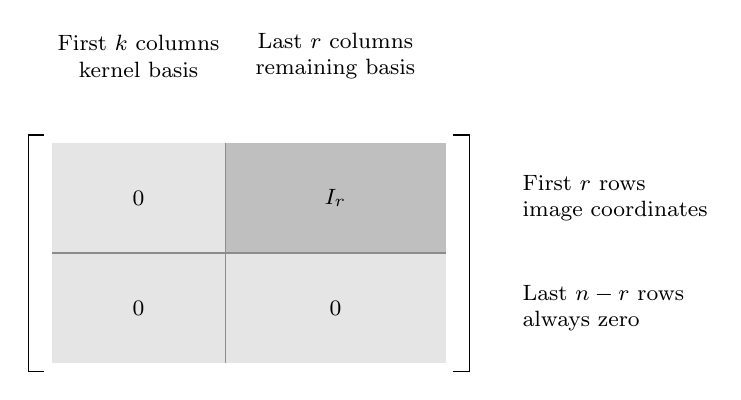
\begin{tikzpicture}[
  x=1mm,y=1mm,font=\footnotesize,line width=0.45pt,
  every node/.style={inner sep=2pt},
  group label/.style={align=center},
  row label/.style={anchor=west,align=left}
]
  \node[group label] at (11,11)
    {First \(k\) columns\\kernel basis};
  \node[group label] at (36,11)
    {Last \(r\) columns\\remaining basis};

  % Leave a gap between the labels and the matrix brackets.
  \fill[black!10] (0,0) rectangle (22,-28);
  \fill[black!25] (22,0) rectangle (50,-14);
  \fill[black!10] (22,-14) rectangle (50,-28);
  \draw[black!45] (22,0) -- (22,-28);
  \draw[black!45] (0,-14) -- (50,-14);
  \draw (-1,1) -- (-3,1) -- (-3,-29) -- (-1,-29);
  \draw (51,1) -- (53,1) -- (53,-29) -- (51,-29);

  \node at (11,-7) {\(0\)};
  \node at (36,-7) {\(I_r\)};
  \node at (11,-21) {\(0\)};
  \node at (36,-21) {\(0\)};

  \node[row label] at (59,-7)
    {First \(r\) rows\\image coordinates};
  \node[row label] at (59,-21)
    {Last \(n-r\) rows\\always zero};
\end{tikzpicture}
